\chapter{ทฤษฎีความรู้และงานที่เกี่ยวข้อง}
\centering{\bf{\textit{(ตัวอย่างเนื้อหาบทที่สอง...)}}} \\
\thaijustify{
    ในบทที่ 2 จะ...
}
\section{ทฤษฎีที่เกี่ยวข้อง}
    \thaijustify{
        ในโครงงานพัฒนาซอฟต์แวร์นี้ ทางกลุ่มได้ทำการศึกษาค้นคว้า...
    }
    \subsection{ทฤษฎีการเขียนโปรแกรมแบบเชิงวัตถุ}
        \thaijustify{
            ทฤษฎีการเขียนโปรแกรมเชิงวัตถุ (Object-Oriented Programming Theory) เป็นแนวคิดในการออกแบบและพัฒนาซอฟต์แวร์ที่เน้นการแบ่งงานออกเป็นองค์ประกอบที่มีลักษณะคล้ายกับวัตถุจริง ๆ ในโลกทั่วไป ถ้าอิงจากวัตถุในชีวิตจริงก็แสดงว่า วัตถุนั้นมีสถานะ (State), พฤติกรรม (Behavior) และความสัมพันธ์ (Relationship) ระหว่างกัน~\cite{booch87} ในการใช้ทฤษฎีเชิงวัตถุในการพัฒนาซอฟต์แวร์ เราสามารถสร้างองค์ประกอบหรือวัตถุที่มีความสมบูรณ์และเป็นรูปแบบสำหรับแก้ปัญหาแต่ละประเภทได้อย่างมีประสิทธิภาพ~\cite{meyer2000}
        }
        \thaijustify{
            การใช้ทฤษฎีเชิงวัตถุมีข้อได้เปรียบหลายประการ เช่นช่วยลดความซับซ้อนของโค้ดหรือทำให้การบำรุงรักษาซอฟต์แวร์ง่ายขึ้น (Maintainability) เพิ่มความยืดหยุ่นในการพัฒนา (Extendability) และเปิดโอกาสในการนำวัตถุที่มีอยู่แล้วในซอฟต์แวร์มาใช้งานใหม่ (Reusability) การแบ่งงานเป็นวัตถุ (หรือ Object) ย่อย ๆ ทำให้โค้ดมีโครงสร้างที่เรียบง่ายและเป็นระเบียบ เพราะฉะนั้นทำให้การทำงานของโปรแกรมเป็นไปอย่างมีประสิทธิภาพและมั่นคง~\cite{meyer2000}
        }
        \begin{figure}[H]
            \centering
            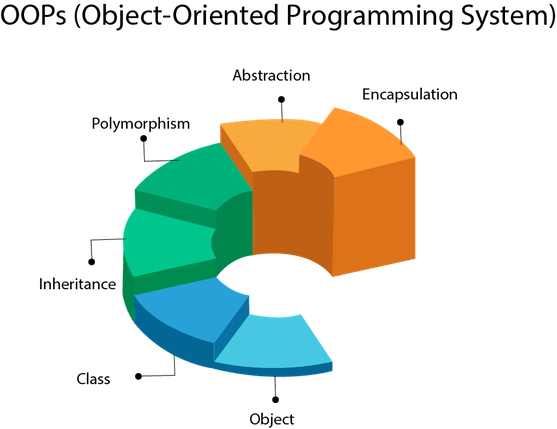
\includegraphics[width=7cm]{chapters/2/figures/oop-programming.png}
            \caption[แผนผังองค์ประกอบของ OOPs]{แผนผังองค์ประกอบของการเขียนโปรแกรมแบบเชิงวัตถุ จาก~\cite{apollo22oop}}
            \label{fig:oop-concept}
        \end{figure}
        \thaijustify{
            องค์ประกอบของระบบโปรแกรมแบบเชิงวัตถุ (\cref{fig:oop-concept}) หรือ Object-Oriented Program System (หรือเรียกโดยย่อว่า OOPs) มีองค์ประกอบดังต่อไปนี้ 
        }
        \subsubsection{การทำ Encapsulation}
            \thaijustify{
                Encapsulation เป็นเหมือนการรวมข้อมูลและฟังก์ชันเข้าด้วยกัน จากงานศึกษาค้นคว้าของ \textit{Nzerue-Kenneth et al.}~\cite{nzeruekenneth23polymorph} เหมือนกับการใส่ไว้ในแคปซูลป้องกัน แนวคิดหลักคือการซ่อนความซับซ้อนของ Objects จากโปรแกรมและผู้ใช้ ทำให้ใช้งานได้ง่ายขึ้น มันคือทั้งหมดที่เกี่ยวกับการซ่อนการทำงานภายในของโค้ดไว้ ดังนั้นจึงไม่ต้องกังวลเกี่ยวกับวิธีการทำงาน แค่ใช้งานอย่างเดียวเท่านั้น
            }
            \begin{figure}[H]
                \centering
                \subfloat[การเปรียบเทียบการทำ Encapsulation กับยาแคปซูล~\cite{raut22encapsule}]{
                    \fbox{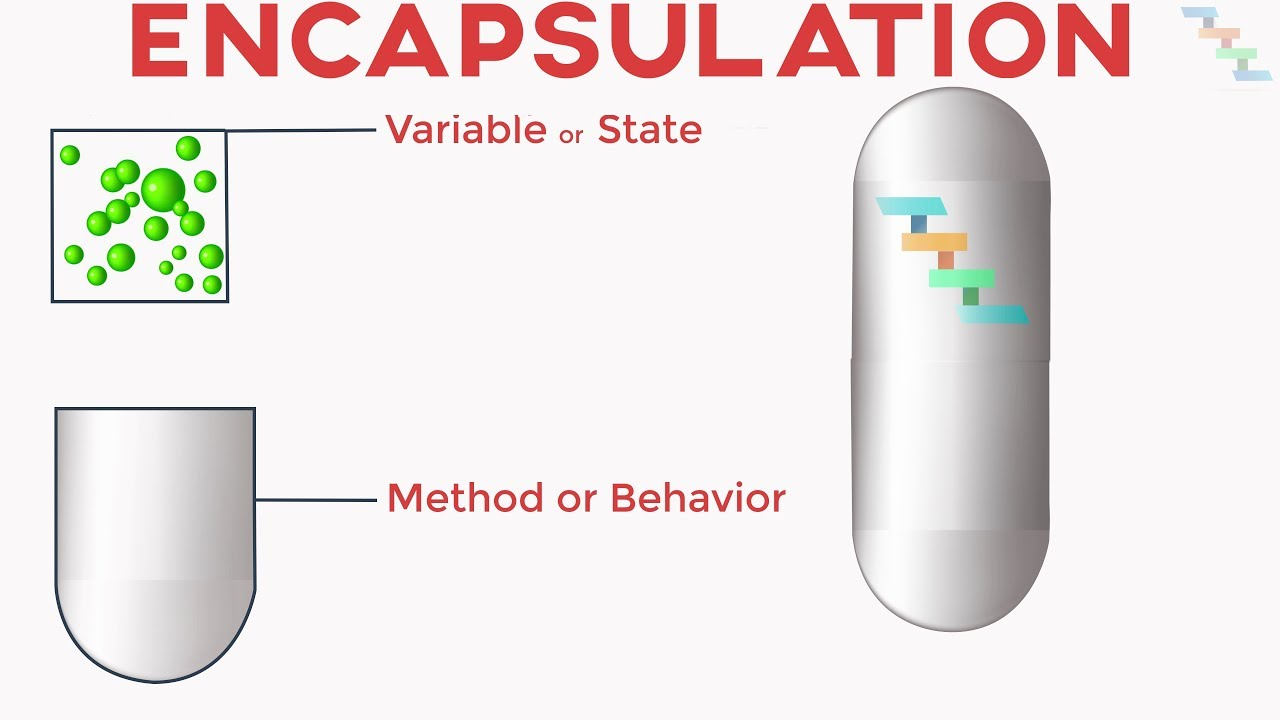
\includegraphics[width=6cm]{chapters/2/figures/oop-encapsulation.png}}
                    \label{fig:oop-encapsulation-capsule}
                }
                \subfloat[การทำ Encapsulation เพื่อปกปิดคุณสมบัติของคลาส~\cite{nishad22encapsulation}]{
                    \fbox{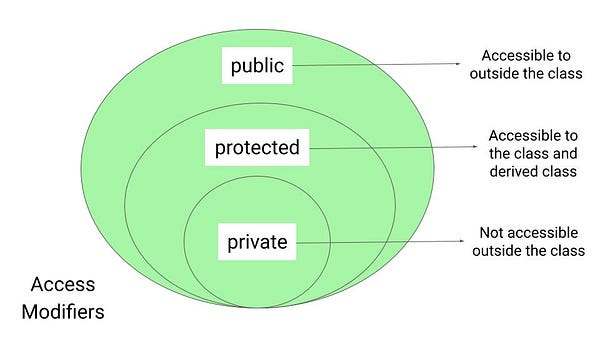
\includegraphics[width=6cm]{chapters/2/figures/oop-encapsulation-detail.jpg}}
                    \label{fig:oop-encapsulation-details}
                } 
                \caption[แผนผังอธิบายการทำ Encapsulation]{แผนผังอธิบายการทำ Encapsulation}
                \label{fig:oop-encapsulation}
            \end{figure}
            \thaijustify{
                จากบทความของ \textit{Raut A.}~\cite{raut22encapsule} ได้เปรียบเทียบหลักการนี้กับแคปซูลที่ปกป้องยาที่อยู่ภายใน ตามในรูปที่~\ref{fig:oop-encapsulation-capsule} การห่อหุ้มของแคปซูลจะปกป้องข้อมูลและฟังก์ชันในโปรแกรม มันเชื่อมโยงโค้ดและข้อมูลที่มันทำงานด้วย สร้างเกราะป้องกันล้อมรอบพวกมัน ด้วยการห่อหุ้ม คุณสามารถจำกัดการเข้าถึงบางส่วนของออบเจ็กต์ โดยให้เฉพาะส่วนอื่น ๆ ของโปรแกรมเข้าถึงสิ่งที่พวกเขาต้องการเท่านั้น เหมือนกับมีตู้จำหน่ายสินค้าอัตโนมัติ คุณไม่สามารถเข้าไปซื้อขนมข้างในได้เว้นแต่คุณจะใช้ปุ่มของเครื่อง ในทำนองเดียวกัน ในการห่อหุ้ม ตัวแปรและฟังก์ชันของวัตถุจะถูกซ่อนไว้และสามารถเข้าถึงได้ผ่านวิธีการเฉพาะภายในคลาสของวัตถุนั้นเท่านั้น
            }
            \thaijustify{
                ดังนั้น การทำ Encapsulation คือทั้งหมดที่เกี่ยวกับการเก็บรักษาสิ่งของต่างๆ ให้ปลอดภัยและซ่อนไว้ตามรูปที่~\ref{fig:oop-encapsulation-details} เช่นเดียวกับยาในแคปซูลหรือของว่างในตู้จำหน่ายสินค้าอัตโนมัติ ช่วยให้โปรแกรมใช้งานและเข้าใจได้ง่ายขึ้นโดยปกป้องการทำงานภายในของโปรแกรมเหล่านั้น~\cite{nishad22encapsulation}
            }
\section{โครงงาน งานวิจัยหรือผลิตภัณฑ์ที่เกี่ยวข้อง}
    เนื่องจาก... กลุ่มเราจึงศึกษา... มาใช้อ้างอิง... นำมาประยุกต์ใช้ใน...
    \subsection{IPST Program Grader}
        \thaijustify{
            \href{https://programming.in.th}{IPST Program Grader} เป็นเว็บไซต์ แอปพลิเคชันที่สร้างขึ้นโดย\textit{สถาบันส่งเสริมการสอนวิทยาศาสตร์และเทคโนโลยี (สสวท.)}~\cite{ipstGrader} ถูกนำมาปรับปรุงใหม่โดยกลุ่มนักเรียนค่ายโอลิมปิกวิชาการคอมพิวเตอร์ในช่วงล่าสุดนี้ เว็บไซต์ดังกล่าวถูกสร้างขึ้นมาเพื่อให้ผู้ใช้สามารถเข้ามาฝึกฝนทักษะการเขียนโปรแกรม เรียนรู้การเขียนโปรแกรม เรียนรู้เกี่ยวกับโครงสร้างข้อมูล และฝึกเขียนอัลกอริทึมที่มีประสิทธิภาพ
        }
        \begin{figure}[H]
            \centering
            \subfloat[หน้าหลักเว็บไซต์ ณ วันที่ 10 ธันวาคม 2562~\cite{ipstGrader}]{
                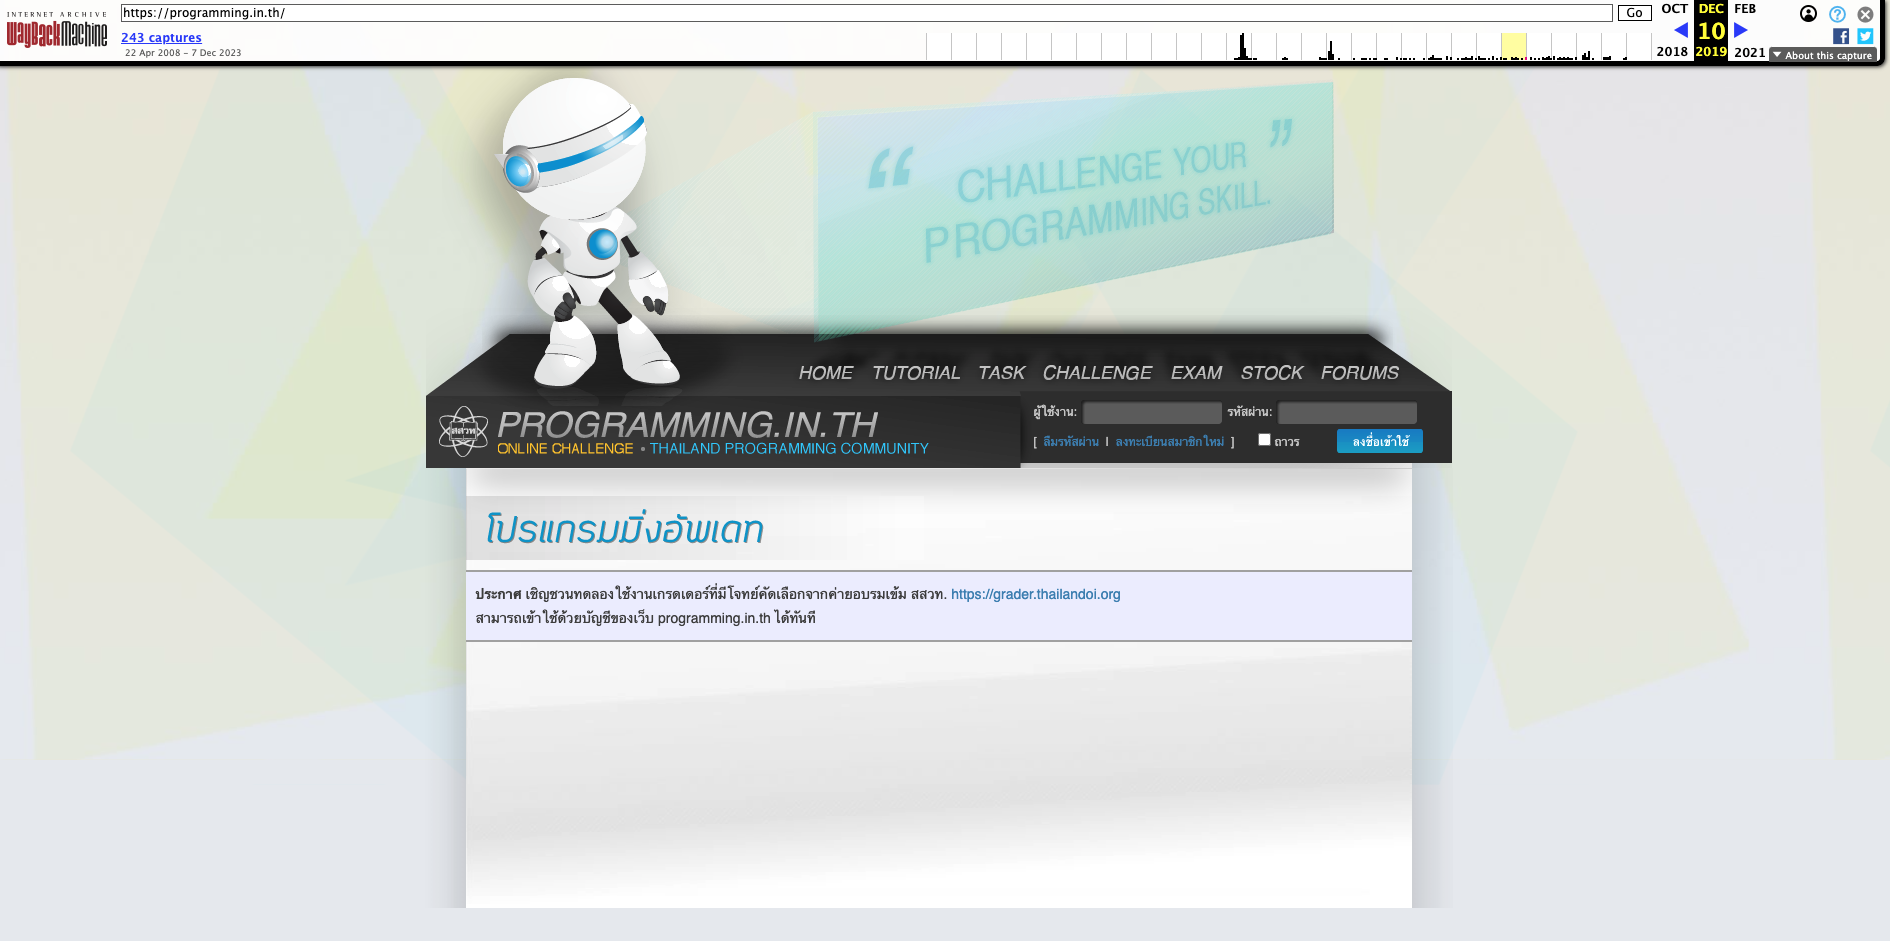
\includegraphics[width=7cm]{chapters/2/figures/old-ipst.png}
                \label{fig:ipst-page-old}
            }
            \subfloat[หน้าหลักเว็บไซต์ ณ ปัจจุบัน]{
                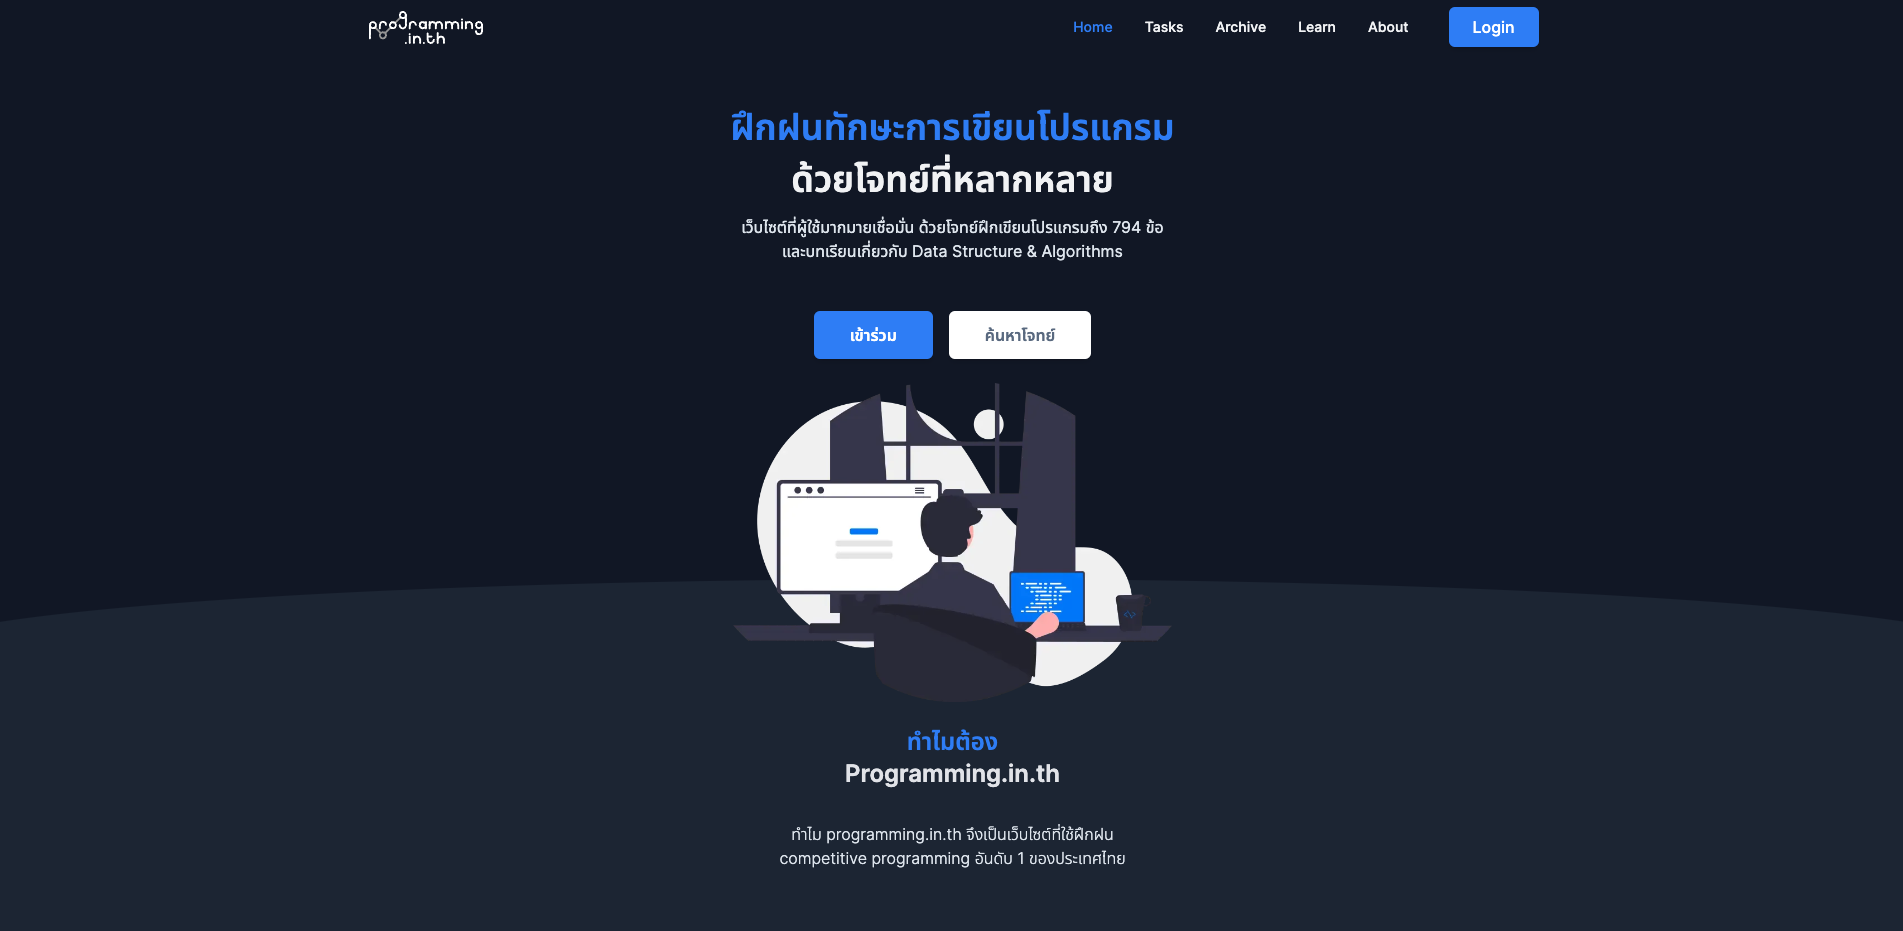
\includegraphics[width=7cm]{chapters/2/figures/current-ipst.png}
                \label{fig:ipst-page-new}
            } 
            \caption[หน้าหลักของ IPST Program Grader]{หน้าหลักของ IPST Program Grader}
            \label{fig:ipst-page}
        \end{figure}
        \thaijustify{
            เว็บไซต์นี้มีฐานข้อมูลโจทย์ปัญหาที่แต่งโดยทางสสวท. ที่ผู้ใช้สามารถกดเลือกเข้าไปทำข้อไหนก็ได้ มีระบบสมัครสมาชิก และมีแหล่งเรียนรู้เพิ่มเติม (Learning resource) สำหรับให้ผู้ใช้ได้เข้าอ่านทำความเข้าใจและเรียนรู้การเขียนโปรแกรม
        }
        \thaijustify{
            เว็บไซต์ดังกล่าวเป็นหนึ่งในแรงบันดาลใจ ต้นฉบับความคิดและต้นแบบซอฟต์แวร์ที่~\cite{nattawat20pgs} ใช้เป็นตัวอย่างในเชิงของแนวคิดในการออกแบบซอฟต์แวร์
        }
        \thaijustify{
                ใน \textit{Jamlongrad et al.}~\cite{nattawat20pgs} ได้มีการวิเคราะห์ สรุปข้อดีและข้อเสียของระบบ แต่เนื่องจากเว็บไซต์ได้มีการเปลี่ยนแปลงในรอบปีที่ผ่านมา คณะผู้จัดทำก็ได้ไปสำรวจการทำงานเว็บไซต์ใหม่อีกรอบหนึ่ง แล้วนำผลสำรวจมาสรุปรวบยอดกับในรายงานดังกล่าว สรุปเป็นผลเป็น~\cref{tbl:ipst-pro-cons} ดังต่อไปนี้
        }
        \begin{table}[H]
            \centering
            \caption{ข้อดีและข้อเสียของระบบ IPST Grader}
            \label{tbl:ipst-pro-cons}
                \begin{tabular}{p{1cm}|p{6cm}|p{6cm}} \hline\hline
                    ข้อที่ & ข้อดี & ข้อเสีย \\ 
                    \hline\hline
                    1. & \RaggedRight{เว็บไซต์มีระบบการตรวจและประเมินผลโปรแกรมที่รวดเร็ว ผู้ใช้สามารถรับรู้ผลได้ทันที}\par & \RaggedRight{เว็บไซต์ไม่สามารถจะใช้งานเครือข่ายเฉพาะได้ เพราะเว็บไซต์ดังกล่าวอยู่ในเครือข่ายสาธารณะ ทำให้เว็บไซต์นี้ไม่สามารถนำมาใช้ในการแข่งขันภายในได้}\par \\ \hline
                    2. & \RaggedRight{ส่วนประสานผู้ใช้ถูกออกแบบมาอย่างดี เพื่อความสะดวกสบายของผู้ใช้}\par & \RaggedRight{ไม่มีระบบสื่อสาร ไม่มีระบบกระทู้สนทนา ไม่มีช่องทางการสื่อสารให้ผู้ใช้ได้คุยปรึกษากันเรื่องโจทย์}\par \\ \hline
                    3. & \RaggedRight{เว็บไซต์มีโจทย์ปัญหาที่หลากหลาย แต่งแต่ระดับง่ายสุด ไปยังระดับการแข่งขันระดับนานาชาติ}\par & \RaggedRight{ผู้ใช้ไม่สามารถเพิ่มโจทย์ปัญหาเองได้ โจทย์ปัญหาถูกควบคุมและเพิ่มโดยผู้ดูแลเว็บเท่านั้น}\par \\ \hline
                    4. & \RaggedRight{เว็บไซต์มีระบบจัดหมวดหมู่โจทย์ปัญหา ทำให้ผู้ใช้หาโจทย์ปัญหาที่ต้องการทำได้ง่าย}\par & \\
                    \hline\hline
                \end{tabular}   
        \end{table}

\section{ภาษาคอมพิวเตอร์เเละเทคโนโลยี}
    \thaijustify{
        หลังจาก... ทางกลุ่มจะอธิบาย... เครื่องมือ เทคโนโลยีและซอฟต์แวร์...
    }
    \subsection{ภาษาคอมพิวเตอร์}
        \thaijustify{
            เพราะ... ทางกลุ่มจึงได้ไปศึกษาหาภาษาคอมพิวเตอร์...
        }
        \subsubsection{ภาษา Go}
            \thaijustify{
                ภาษา Go หรือที่รู้จักกันอย่างแพร่หลายว่า Golang เป็นภาษาโปรแกรมเปิดต้นทางที่พัฒนาโดยทีมนักพัฒนาซอฟต์แวร์ที่ Google โดยรวมถึง Robert Griesemer, Rob Pike, และ Ken Thompson เหล่านักพัฒนาที่ในไม่กี่ทศวรรษก่อน พัฒนาภาษา C ขึ้นมา ภาษา Go นั้นถูกออกแบบขึ้น เพื่อแก้ไขข้อจำกัดของภาษาโปรแกรมเดิมที่มีอยู่แล้วทั้งในด้านประสิทธิภาพ (Efficiency) ความเรียบง่าย (Simplicity) และการสนับสนุนการทำงานพร้อมกัน (Concurrency มีไวยากรณ์ (Syntax) ที่กระชับ การกำหนดประเภท (Type) ที่แข็งแรง พร้อมทั้งระบบจัดการทรัพยากรขยะของโปรแกรม (Garbage Collection) ที่มีประสิทธิภาพ~\cite{pike12go, donovan15go}
            }
            \thaijustify{
                จากความเห็นของ \textit{Pike R.} ใน~\cite{pike12go, pike12godev} หนึ่งในลักษณะที่ดีเด่น Go คือการให้ความสำคัญกับความเรียบง่ายและความอ่านง่าย ทำให้เป็นทางเลือกที่ยอดเยี่ยมสำหรับทั้งผู้เริ่มต้นและนักพัฒนาที่มีประสบการณ์มาก มันนำเสนอแนวทางที่มีความเรียบง่าย ป้องกันความซับซ้อนที่ไม่จำเป็น และมีไวยากรณ์ที่ถูกต้องและโดดเด่น ภาษานี้รวมถึงคุณสมบัติที่สนับสนุนการทำงานพร้อมกันที่ซึ่งช่วยให้นักพัฒนาสามารถเขียนแอปพลิเคชันที่มีประสิทธิภาพและมีขนาดใหญ่ได้
            }
            \thaijustify{
                การทำงานพร้อมกันหรือ Concurrency ก็เป็นแข็งสำคัญของ Go อย่างหนึ่ง การทำ Concurrency ในภาษา ทำผ่าน Channel และ GoRoutines ซึ่งเป็น Thread ที่ Light-weighted ทำให้สามารถสร้างโปรแกรมที่ทำงานพร้อมกันได้โดยไม่มีความซับซ้อน~\cite{donovan15go}
            }
            \thaijustify{
                เนื่องจาก ภาษา Go นั้นกำลังได้รับความนิยมในหลาย ๆ ด้าน ณ ปีการศึกษานี้เช่น การสร้างหรือพัฒนาเว็บไซต์ เว็บแอปพลิเคชัน, การสร้างระบบบริการ Cloud, การสร้างซอฟต์แวร์ระบบที่มีประสิทธิภาพ เป็นต้น ภาษา Go เป็นภาษาที่ใช้งานง่าน และสามารถรันโปรแกรมที่อาศัยการทำงานหรือประมวลแบบ Parallel และ Concurrent~\cite{golangorg} ด้วยเหตุนี้บริษัทใหญ่หลายบริษัทในยุคใหม่ที่มีระบบซอฟต์แวร์ที่ใหญ่ จึงนิยมใช้ภาษาดังกล่าว แล้วเนื่องด้วยสมาชิกในกลุ่มคณะผู้จัดทำได้มีโอกาสไปฝึกงานบริษัทที่ใช้ภาษาดังกล่าว จึงเห็นเป็นโอกาสนำความรู้และความเข้าใจมาประยุกต์ในโครงงานนี้
            }
    \subsection{เครื่องมือและซอฟต์แวร์โครงสร้างพื้นฐาน}
        เพราะ... กลุ่มเราจึงได้มีการค้นคว้า...
        \subsubsection{เว็บเฟรมเวิร์ค React}
            \thaijustify{
                React เป็นไลบรารี JavaScript ที่ถูกพัฒนาขึ้นโดย Facebook สำหรับสร้าง User Interface (UI) ที่ได้รับความนิยมอย่างแพร่หลายในการพัฒนาเว็บแอปพลิเคชัน (web applications)~\cite{flanagan20js}
            }
            \begin{figure}[H]
                \centering
                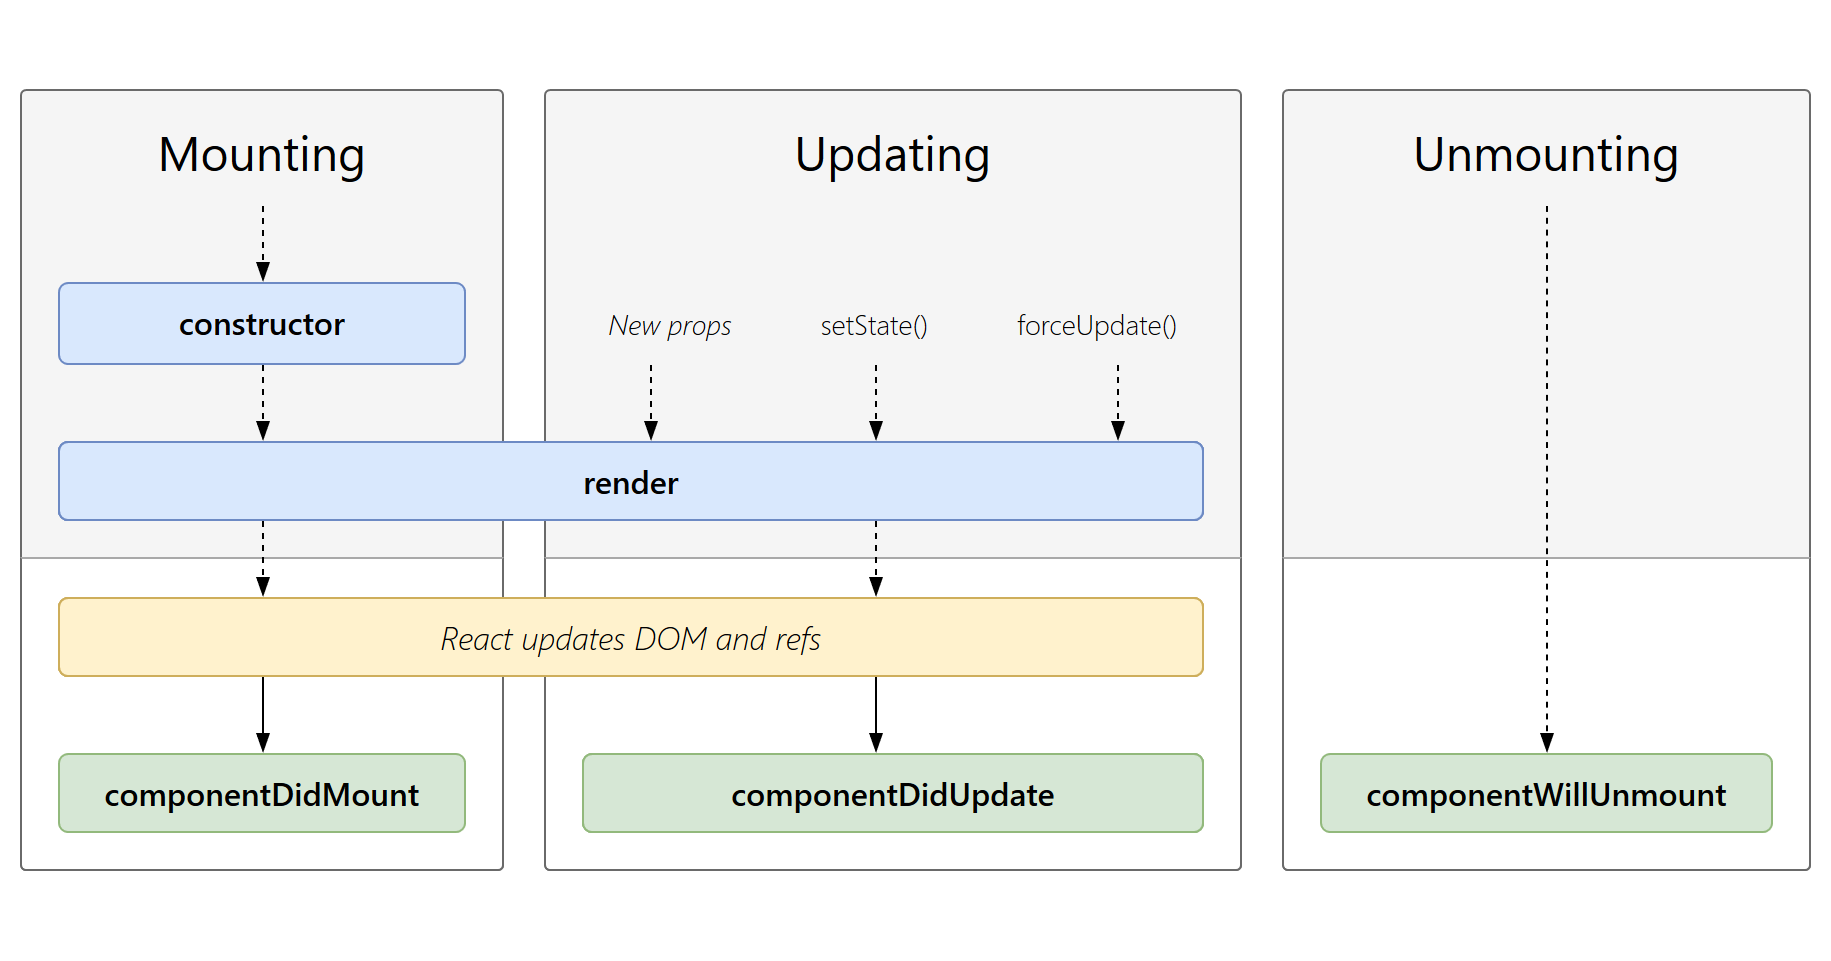
\includegraphics[width=12cm]{chapters/2/figures/react-lifecycle.png}
                \caption[วัฏจักรการทำงานของ React]{วัฎจักรการ Render, Mount-Unmount และ Update ของ React (React Lifecycle) จาก~\cite{reactcycles}}\label{fig:lit-react}
            \end{figure}
            \thaijustify{
                React ให้เครื่องมือและโครงสร้างที่สำหรับการสร้างชิ้นส่วนประกอบของส่วนประสานงานผู้ใช้หรือ UI components ได้หลากหลายและมีประสิทธิภาพ~\cite{crockford08js} หนึ่งในข้อได้เปรียบของ React อยู่ที่การใช้ Virtual DOM ที่ช่วยเพิ่มประสิทธิภาพของการ Render องค์ประกอบของ UI และการสร้างแอปพลิเคชันที่มีประสิทธิภาพและสามารถบริหารจัดการ State ของแอปพลิเคชันได้ง่าย~\cite{flanagan20js}...
            }
\section{สรุปการศึกษาค้นคว้า}
    \thaijustify{
        จาก... คณะผู้จัดทำได้นำหลักการ วิทยาการ และเทคโนโลยี นำไปประยุกต์...
    }
    \subsection{การประยุกต์ใช้ทฤษฎีและหลักการ}
        \thaijustify{
            หลักการเขียนโปรแกรมเชิงวัตถุหรือ OOPs จาก~\cite{booch87, meyer2000, apollo22oop} เป็นหลักการเขียนโปรแกรมที่มีประโยชน์อย่างมาก สามารถที่จะทำให้ผู้พัฒนาซอฟต์สามารถที่จะออกแบบและสร้างที่มีความต้องการและมีการทำงานขึ้นมาได้อย่างง่ายได้ หากใช้ร่วมกับแนวคิดการออกแบบแยกข้อกังวลและแยกความรับผิดชอบหรือ SoC นั้น จะทำให้ระบบซอฟต์แวร์มีส่วนการทำงานที่ถูกนิยามและวางไว้อย่างชัดเจน มีหน้าถ้าหากส่วนใดเกิดปัญหาขึ้นมาในส่วนใดของซอฟต์แวร์ ก็จะสามารถที่จะสืบหาที่มาของปัญหาได้อย่างรวดเร็วเพราะผู้พัฒนาก็จะรู้ว่าส่วนใดในซอฟต์แวร์ที่รับผิดชอบหน้าที่นั้น ๆ~\cite{nattawat20pgs, wikipedia04soc}
        }
        \thaijustify{
            แต่จากที่ได้ศึกษาจาก~\cite{thomas99pragmatic, fowler13oop, nattawat20pgs} ถ้าหากใช้หลักการเขียนโปรแกรมเชิงวัตถุมากเกินควรจำเป็น ก็ย่อมทำให้เกิดผลเสียได้ อย่างซอฟต์แวร์ที่เขียนขึ้นมามีความซับซ้อนมากไป มีขั้นตอนในการแก้ปัญหาใดปัญหาหนึ่งที่ยุ่งยากหลายขั้นตอน วัตถุหนึ่งต้องส่งข้อมูลชุดหนึ่งไปแก้ในวัตถุชุดต่อ ๆ ไป ทำให้การแก้ปัญหาง่าย ๆ กลายเป็นเรื่องยากหรือเรียกว่าเป็นการแก้ปัญหาที่~\textit{Over-engineered} มาก เห็นได้อย่างชัดเจนจากการศึกษาและวิเคราะห์ระบบของ~\cite{nattawat20pgs}...
        }
    \subsection{การประยุกต์ใช้เครื่องมือและเทคโนโลยี}
       \thaijustify{
            ...
        }
\pagebreak